\documentclass[twoside]{article}
\usepackage{graphics}
\usepackage{amsmath}
\usepackage{amssymb}
\usepackage{epsfig}
\usepackage{kotex}
\setlength{\oddsidemargin}{0.25 in}
\setlength{\evensidemargin}{-0.25 in}
\setlength{\topmargin}{-0.6 in}
\setlength{\textwidth}{6.5 in}
\setlength{\textheight}{8.5 in}
\setlength{\headsep}{0.75 in}
\setlength{\parindent}{0 in}
\setlength{\parskip}{0.1 in}

%
% The following commands set up the lecnum (lecture number)
% counter and make various numbering schemes work relative
% to the lecture number.
%
\newcounter{lecnum}
\renewcommand{\thepage}{\thelecnum-\arabic{page}}
\renewcommand{\thesection}{\thelecnum.\arabic{section}}
\renewcommand{\theequation}{\thelecnum.\arabic{equation}}
\renewcommand{\thefigure}{\thelecnum.\arabic{figure}}
\renewcommand{\thetable}{\thelecnum.\arabic{table}}
\DeclareMathOperator*{\argmax}{argmax}
\DeclareMathOperator*{\argmin}{argmin}

%
% The following macro is used to generate the header.
%
\newcommand{\lecture}[4]{
   \pagestyle{myheadings}
   \thispagestyle{plain}
   \newpage
   \setcounter{lecnum}{#1}
   \setcounter{page}{1}
   \noindent
   \begin{center}
   \framebox{
      \vbox{\vspace{2mm}
    \hbox to 6.28in { {\bf EE 531 Statistical Learning Theory
                        \hfill Spring 2017} }
       \vspace{4mm}
       \hbox to 6.28in { {\Large \hfill Lecture #1: #2  \hfill} }
       \vspace{2mm}
       \hbox to 6.28in { {\it Lecturer: #3 \hfill Scribe: #4} }
      \vspace{2mm}}
   }
   \end{center}
   \markboth{Lecture #1: #2}{Lecture #1: #2}
   {\bf Disclaimer}: {\it These notes have not been subjected to the
   usual scrutiny reserved for formal publications.  They may be distributed
   outside this class only with the permission of the Instructor.}
   \vspace*{4mm}
}

%
% Convention for citations is authors' initials followed by the year.
% For example, to cite a paper by Leighton and Maggs you would type
% \cite{LM89}, and to cite a paper by Strassen you would type \cite{S69}.
% (To avoid bibliography problems, for now we redefine the \cite command.)
% Also commands that create a suitable format for the reference list.
\renewcommand{\cite}[1]{[#1]}
\def\beginrefs{\begin{list}%
        {[\arabic{equation}]}{\usecounter{equation}
         \setlength{\leftmargin}{2.0truecm}\setlength{\labelsep}{0.4truecm}%
         \setlength{\labelwidth}{1.6truecm}}}
\def\endrefs{\end{list}}
\def\bibentry#1{\item[\hbox{[#1]}]}

%Use this command for a figure; it puts a figure in wherever you want it.
%usage: \fig{NUMBER}{SPACE-IN-INCHES}{CAPTION}
\newcommand{\fig}[3]{
			\vspace{#2}
			\begin{center}
			Figure \thelecnum.#1:~#3
			\end{center}
	}
% Use these for theorems, lemmas, proofs, etc.
\newtheorem{theorem}{Theorem}[lecnum]
\newtheorem{lemma}[theorem]{Lemma}
\newtheorem{proposition}[theorem]{Proposition}
\newtheorem{claim}[theorem]{Claim}
\newtheorem{corollary}[theorem]{Corollary}
\newtheorem{definition}[theorem]{Definition}
\newenvironment{proof}{{\bf Proof:}}{\hfill\rule{2mm}{2mm}}

% **** IF YOU WANT TO DEFINE ADDITIONAL MACROS FOR YOURSELF, PUT THEM HERE:

\begin{document}
%FILL IN THE RIGHT INFO.
%\lecture{**LECTURE-NUMBER**}{**DATE**}{**LECTURER**}{**SCRIBE**}
\lecture{13}{April 25}{Chang D. Yoo}{Cho Seong Jin}
%\footnotetext{These notes are partially based on those of Nigel Mansell

% **** YOUR NOTES GO HERE:

% Some general latex examples and examples making use of the
% macros follow.  
%**** IN GENERAL, BE BRIEF. LONG SCRIBE NOTES, NO MATTER HOW WELL WRITTEN,
%**** ARE NEVER READ BY ANYBODY.

\section{Regularization methods of linear regression}

만약 $\mathbf{\Phi}^T (\mathbf{X})\mathbf{\Phi}(\mathbf{X})$이 singular 하면, diagonal matrix ($\lambda I$)를 더함으로써 non-singular하게 만들 수 있고, 따라서 다음과 같이 $\mathbf{w}$를 구할 수 있다.
$$\mathbf{w} = (\lambda I + \mathbf{\Phi}^T \mathbf{\Phi})^{-1} \mathbf{\Phi}^T \mathbf{y}$$
이 식은 RSS에 다음과 같이 항을 추가함으로써 얻을 수 있다.
$$(\mathbf{y} - \mathbf{\Phi}(\mathbf{X})\mathbf{w})^T (\mathbf{y} - \mathbf{\Phi}(\mathbf{X})\mathbf{w}) + \lambda \mathbf{w}^T \mathbf{w}$$
여기에서 두번 째 항($\lambda \mathbf{w}^T \mathbf{w}$)은 regularization(stabilization) term으로 $\mathbf{w}$가 너무 커지는 것에 제약을 가하여(weight decay) overfitting을 막는 역할(overfitting control)을 한다. 또 다른 표현으로 parameter shrinkage라고도 한다. linear regression에서 regularization은 다음과 같이 일반적으로 표현할 수 있는데,
$$\min_{\mathbf{w}} \max_{\lambda} \left[ \sum_{i=1}^{N} (y_i - \mathbf{w}^T \mathbf{\phi} (x_i))^2 + \lambda (\sum_{j=1}^{p} |w_j|^q -s)\right]$$
이는
$$\sum_{j=1}^{p} |w_j|^q \le s$$
조건에서
$$\min_{\mathbf{w}} \sum_{i=1}^{N} (y_i - \mathbf{w}^T \mathbf{\phi} (x_i))^2$$
를 구하는 것과 같다. 여기에서 $q=1$이면 lasso regression, $q=2$이면 ridge regression이라 한다. 두 regularization에 대한 graphical interpretation을 Figure \ref{fig:13-3}에 표현하였다. 그림을 보면 regularization과 RSS의 접점에서 $\mathbf{w}^*$가 얻어진다. 그림에서 보는 바와 같이 $q=1$이면, 각 축에서 접점이 얻어질 가능성이 높아지고 이는 sparse한 파라미터 벡터를 얻게 한다.

\begin{figure}[h]
	\centering
	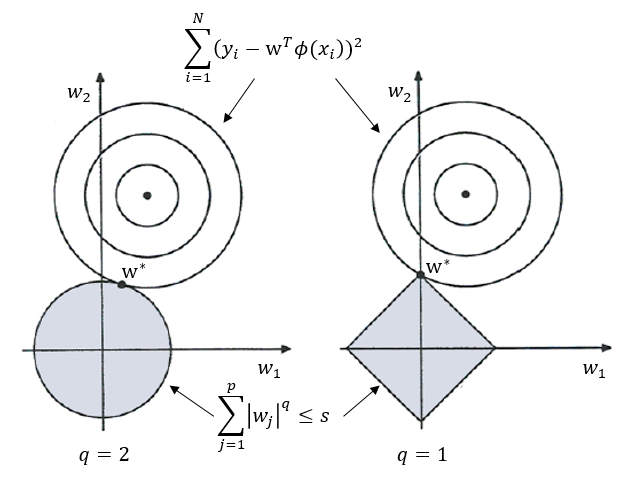
\includegraphics[width=0.5\linewidth]{13-3}
	\caption{Graphical interpretation of regularization.}
	\label{fig:13-3}
\end{figure}

linear regression에서 Bayesian treatment를 이용하면 MLE (maximum likelihood estimation)의 overfitting 문제를 해결할 수 있다. MLE에서는 $p(\mathbf{y}|\mathbf{w})$만을 최대로 하기 때문에, $\mathbf{w}$의 분포와 상관없이 트레이닝 데이터에 최적화된 $\mathbf{w}^*$를 구하는 반면, MAP (maximum a posterior)에서는 $p(\mathbf{w})$가 동시에 적용되기 때문에, $\mathbf{w}$가 prior distribution에 의해 제약을 받고, 이는 MLE가 overfitting되지 않도록 regularization 역할을 한다. 다음의 예를 보자.

\textbf{Example: Polynomial Curve Fitting}\\
target labels $\mathbf{y} = (y_1, y_2, \ldots, y_N)$가 $x \in [0, 1]$에서 $y=\sin(2 \pi x) + \epsilon$으로 주어졌을 때, hypothesis를 다음과 같이 $x$의 polynomial로 정하고,
$$f(x, \mathbf{w}) = \sum_{j=0}^{M} w_j x^j = w_0 + w_1 x + w_2 x^2 + \cdots + w_M x^M$$
loss를 다음과 정의하면,
$$L(\mathbf{w}) = \frac{1}{2} \sum_{i=1}^{N} (y_i - f(x_i, \mathbf{w}))^2$$
$\mathbf{w}^* = \argmin_\mathbf{w} L(\mathbf{w})$가 된다. Figure \ref{fig:13-4}는 $N=10$일 때, $M$에 따른 polynomial curve의 예이다. 그림을 보면 $M=9$일 때, overfitting 된 것을 확인할 수 있다.

\begin{figure}[h]
	\centering
	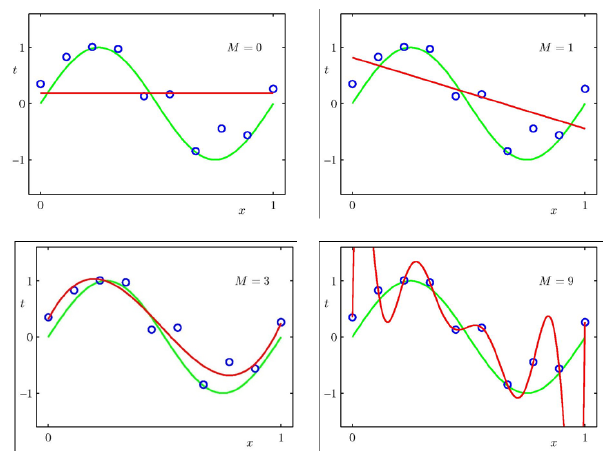
\includegraphics[width=0.5\linewidth]{13-4}
	\caption{Plots of polynomials having various orders M with 10 samples.}
	\label{fig:13-4}
\end{figure}

그런데 실제 target function인 sine 함수는 다음과 같은 Taylor series를 갖기 때문에,
$$\sin (x) \approx x - \frac{x^3}{3!} + \frac{x^5}{5!} - \frac{x^7}{7!} + \frac{x^9}{9!} - \cdots$$
$M=9$에서 잘 적용될 것 같지만, 예에서 overfitting 된 이유는 샘플의 개수가 model complexity에 비해 적기 때문에 발생한 것이다. Figure \ref{fig:13-5}를 보면 $N=100$일 때, $M=9$에서 overfitting 되지 않고 잘 적용되는 것을 확인할 수 있다. 따라서, 트레이닝 샘플의 개수를 증가시키면 overfitting 문제를 줄일 수 있다.

\begin{figure}[h]
	\centering
	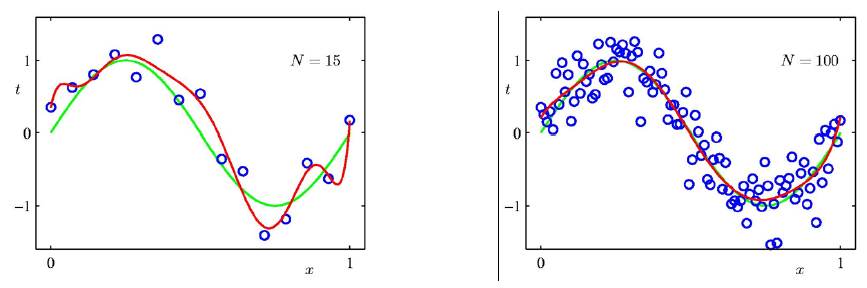
\includegraphics[width=0.7\linewidth]{13-5}
	\caption{$M=9$ ploynomial for $N=15$, $N=100$}
	\label{fig:13-5}
\end{figure}

그러나 샘플 개수는 한정되어 있을 수 있다. 따라서 이 문제를 해결하기 위해 regularization term을 추가하고, 이는 적은 샘플로도 overfitting을 방지할 수 있게 한다. 즉, loss에 다음과 같이 regularization term을 추가하여 $\mathbf{w}^*$를 구하면, overfitting을 줄일 수 있다. Figure \ref{fig:13-6}을 보면 $\lambda$가 적절한 값을 갖을 때, overfitting되지 않는 것을 확인할 수 있다. 이 때, $\lambda$가 너무 크면 regularization term이 너무 크게 작용하여 underfitting 될 수 있기 때문에, cross-validation을 통해 적절한 값을 찾아야 한다.
$$\tilde{L}(\mathbf{w}) = \frac{1}{2} \sum_{i=1}^{N} (y_i - f(x_i, \mathbf{w}))^2 + \frac{\lambda}{2} |\!| \mathbf{w} |\!|^2$$

\begin{figure}[h]
	\centering
	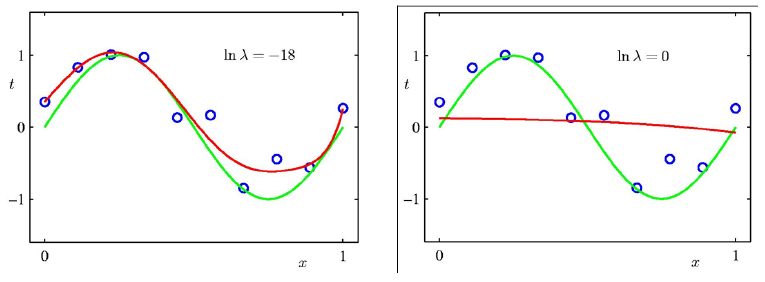
\includegraphics[width=0.7\linewidth]{13-6}
	\caption{$M=9$ polynomial for $\ln \lambda=-18$, $\ln \lambda=0$}
	\label{fig:13-6}
\end{figure}


\end{document}




